\documentclass[conference]{IEEEtran}
\usepackage{cite}
\usepackage{amsmath,amssymb,amsfonts}
\usepackage{graphicx}
\usepackage{textcomp}
\usepackage{xcolor}
\usepackage{booktabs}
\usepackage{multirow}
\usepackage{tikz}
\usepackage{pgfplots}
\pgfplotsset{compat=1.18}
\usepackage{float}

\title{Food Waste Reduction Platform: A Geospatially Constrained Mobile Application for Real-Time Surplus Redistribution in Bogotá}

\author{
\begin{tabular}{cc}
Luna Alejandra Sandoval Rodríguez & Cristian Camilo Bonilla Lizarazo \\
\textit{Project Lead} & \textit{Frontend Developer} \\
Universidad Distrital & Universidad Distrital \\
20241020053 & 20241020015 \\[0.5cm]

Nicolás Rodríguez Granados & Juan Sebastián Bravo Rojas \\
\textit{Backend Developer} & \textit{Database Specialist} \\
Universidad Distrital & Universidad Distrital \\
20241020037 & 20241020004 \\
\end{tabular}
}

\begin{document}

\maketitle

\begin{abstract}
In Colombia, tons of food are wasted annually. Amid a global food loss and waste crisis (which exacerbates environmental damage and food insecurity), this underscores the urgent need for collaborative digital platforms that reduce coordination barriers between donors and recipients. Therefore, this document proposes a mobile application that connects local cafes and restaurants with students, charities, and citizens in Bogotá through geolocation, real-time notifications, and priority rules for verified organizations within a constrained geographic radius. This aims to achieve quantifiable reductions in waste, greater social equity, and alignment with the principles of the circular economy.
\end{abstract}

\begin{IEEEkeywords}
Food waste reduction, real-time matching, geospatial systems, mobile applications, resource allocation, urban surplus redistribution, circular economy, system design, Colombia
\end{IEEEkeywords}

\section{Introduction}
Food waste represents one of the greatest environmental, economic, and social challenges in Colombia. According to the Food Waste Index Report 2021 by the United Nations Environment Programme (UNEP), the country generates approximately 9.7 million tons of food lost or wasted annually, an amount sufficient to feed the entire population of Bogotá \cite{unep2021}.

In Bogotá, local cafeterias and restaurants produce significant quantities of daily surpluses suitable for human consumption, but the lack of rapid coordination and the short shelf life of food cause a large portion to end up in the trash. This situation exacerbates environmental damage (CO$_2$ equivalent emissions), food insecurity, and social inequality, especially in vulnerable communities and among students. In the university context, cafeterias and local restaurants near university areas generate surplus recurrently, but without an efficient digital mechanism that enables immediate redistribution.

In 2024, the Alcaldía of Bogotá launched the initiative ``Yo Contribuyo, No Desperdicio'', recognizing the importance of coordinating efforts among different entities to address the problem collectively \cite{bogota2024}. At the international level, platforms such as OLIO \cite{olio2024} and the Colombian startup EatCloud have demonstrated the potential of mobile applications to reduce waste \cite{eatcloud2025}; however, none are specifically designed for university environments with strict geographic constraints.

This work proposes a mobile application for food waste reduction specifically designed for a spatial radius near the Faculty of Engineering of the Universidad Distrital Francisco José de Caldas. The platform connects local cafeterias and restaurants in real time with students, community members, and foundations through a matching algorithm based on proximity (maximum radius of 3\,km), priority for verified organizations, and tiered notifications. The system is strictly limited to an operational radius of 3\,km around the campus (Carrera 8 \#40-62), operates exclusively within the same day (publication 2-4 hours before closing and pickup within 1-3 hours), and focuses solely on digital coordination, leaving physical logistics and quality verification to the users. In this way, it aims to overcome the limitations identified in existing solutions and generate a measurable impact on waste reduction, social equity, and the principles of the circular economy.

Food waste represents one of the greatest environmental, economic, and social challenges in Colombia. According to the Food Waste Index Report 2021 by the United Nations Environment Programme (UNEP), the country generates approximately 9.7 million tons of food lost or wasted annually, an amount sufficient to feed the entire population of Bogotá \cite{unep2021}. 

In Bogotá, local cafeterias and restaurants produce significant quantities of daily surpluses suitable for human consumption, but the lack of rapid coordination and the short shelf life of food cause a large portion to end up in the trash. This situation exacerbates environmental damage (CO$_2$ equivalent emissions), food insecurity, and social inequality, especially in vulnerable communities and among students. In the university context, cafeterias and local restaurants near university areas generate surplus recurrently, but without an efficient digital mechanism that enables immediate redistribution.

In 2024, the 'Alcaldía' of Bogotá launched the initiative ``Yo Contribuyo, No Desperdicio'', recognizing the importance of coordinating efforts among different entities to address the problem collectively \cite{bogota2024}. At the international level, platforms such as OLIO \cite{olio2024} and the Colombian startup EatCloud have demonstrated the potential of mobile applications to reduce waste\cite{eatcloud2025}; however, none are specifically designed for university environments with strict geographic constraints.

This work proposes a mobile application for food waste reduction specifically designed for a spatial radius near the Faculty of Engineering of the Universidad Distrital Francisco José de Caldas. The platform connects local cafeterias and restaurants in real time with students, community members, and foundations through a matching algorithm based on proximity (maximum radius of 3\,km), priority for verified organizations, and tiered notifications. The system is strictly limited to an operational radius of 3\,km around the campus (Carrera 8 \#40-62), operates exclusively within the same day (publication 2-4 hours before closing and pickup within 1-3 hours), and focuses solely on digital coordination, leaving physical logistics and quality verification to the users. In this way, it aims to overcome the limitations identified in existing solutions and generate a measurable impact on waste reduction, social equity, and the principles of the circular economy.


\section{Methods and Materials}
\subsection{System Architecture}
The proposed platform follows a four-layer architecture designed to separate concerns and support real-time coordination between donors and recipients. Figure~\ref{fig:architecture} illustrates the full system design.

\begin{figure}[htbp]
  \centering
  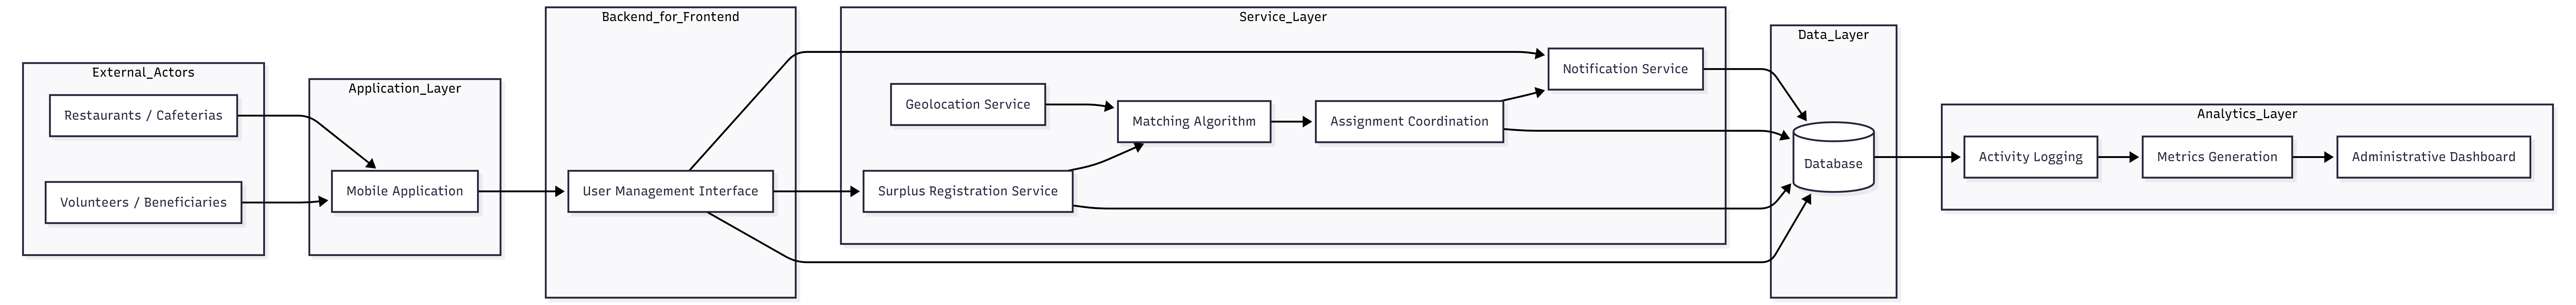
\includegraphics[width=\columnwidth]{System-Architecture-Change (1).png}
  \caption{System architecture of the proposed food surplus redistribution platform.}
  \label{fig:architecture}
\end{figure}

The External Actors layer comprises restaurants and cafeterias as donors that register surplus inventory, together with volunteers and beneficiaries—including verified NGOs, student groups, and individual citizens—who claim available donations. The Application Layer hosts the mobile application and user management interface as the single point of interaction for all user types. It handles authentication, role assignment, and geographic eligibility verification.

The Service Layer forms the core processing tier with the Surplus Registration Service, Geolocation Service, Matching Algorithm, Assignment Coordination module, and Notification Service. The Data Layer uses a centralized relational database for persistence, while the Analytics Layer enables continuous impact reporting and optimization.

\subsection{Matching and Priority Algorithm}
The core of the platform is a priority-based matching algorithm implemented as a dynamic priority queue. When a donor publishes a new surplus listing, the algorithm first queries the Geolocation Service to identify all eligible recipients within the strict 3 km radius using PostGIS geospatial functions. It then computes a composite priority score for each candidate using three weighted factors: organizational verification status (highest for verified NGOs and foundations), historical pickup reliability, and geographic proximity (inverse distance).

Candidates are sorted according to this score, and the system sends tiered push notifications sequentially with a 15-minute response window per tier before cascading to the next. Upon mutual confirmation of pickup (via photo or QR scan), the listing is locked and removed from the active pool. This mechanism prioritizes organizations serving vulnerable populations while preserving efficiency and fairness. The algorithm exhibits $O(n \log n)$ average complexity thanks to priority queue operations, remaining suitable for real-time execution even with hundreds of concurrent users.

\subsection{Operational Constraints and Main Components}
To guarantee food safety, freshness, and logistical feasibility, the platform enforces strict boundaries defined in the Workshop 1 systems analysis. Listings may only be published 2--4 hours before the donor’s closing time, and pickups must occur within 1--3 hours. All listings expire automatically at midnight to ensure same-day redistribution only. The system deliberately excludes physical transportation, quality verification, and economic transactions, leaving those responsibilities to the participating parties.

The main components of the platform, as identified in the systems analysis, are the Mobile Application (frontend for publication, browsing, and notifications), the Cloud Server with relational database (PostgreSQL + PostGIS for persistence and geospatial queries), and the Intelligence Engine (matching algorithm). The primary processes follow an input-process-output model: suppliers register surplus items as input, the system performs validation, geolocation filtering, and priority matching as process, and it delivers successful redistributions together with impact metrics as output. These components and processes ensure end-to-end traceability and support continuous performance monitoring.

\subsection{Technology Stack}
The mobile application is developed using React Native for cross-platform support on Android and iOS, which is relevant given the Android-dominant market in Colombia. Backend services are implemented with Node.js exposing RESTful APIs. PostgreSQL with the PostGIS extension supports geospatial radius queries. Firebase Cloud Messaging (FCM) powers the real-time push notification pipeline. The stack is containerized with Docker and deployed on a cloud provider to ensure availability during peak usage windows.

\subsection{Evaluation Methodology and Sensitivity Analysis}
System effectiveness will be assessed through an eight-week pilot deployment within the operational radius. Quantitative metrics include total kilograms redistributed, successful matches per week, average publication-to-pickup time, and notification response rates by priority tier. A post-pilot survey using a 5-point Likert scale will evaluate usability and perceived impact.

A sensitivity analysis was performed on the simulation by varying key parameters (number of suppliers, daily surplus per supplier, and user response rates). Results show that the redistribution rate remains robust even with ±20\% variation in participation, confirming the system’s resilience to realistic fluctuations in adoption.

\subsection{System Architecture}

The proposed platform follows a four-layer architecture designed to separate concerns and support real-time coordination between donors and recipients. Figure~\ref{fig:architecture} illustrates the full system design.

\begin{figure}[htbp]
  \centering
  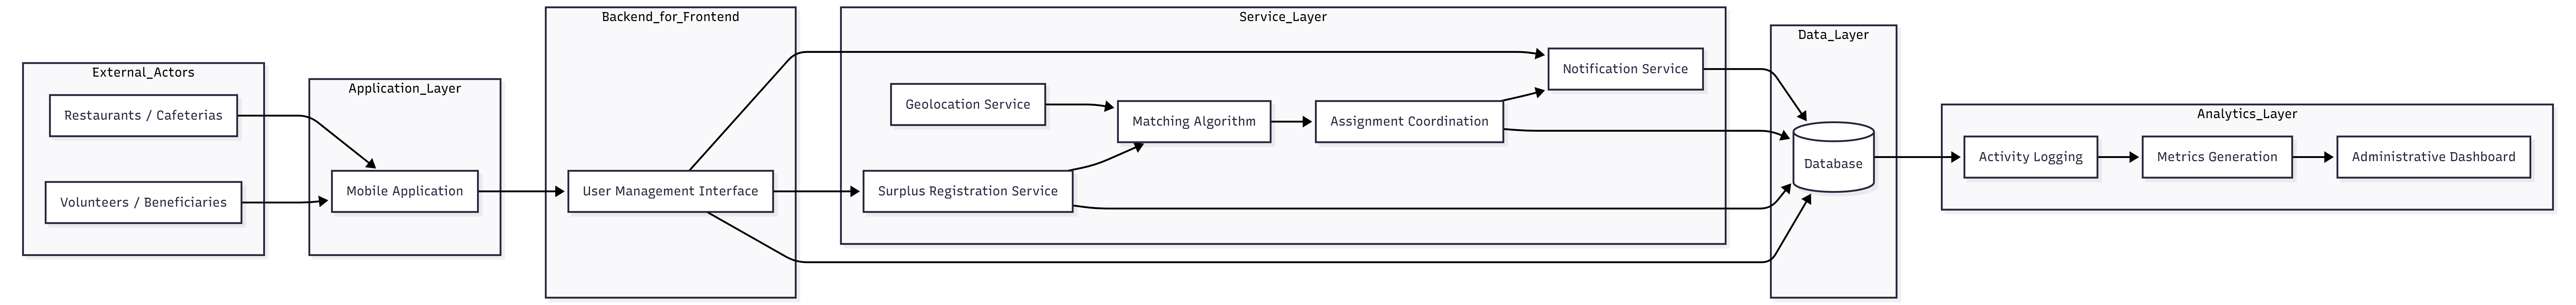
\includegraphics[width=\columnwidth]{System-Architecture-Change (1)}
  \caption{System architecture of the proposed food surplus redistribution platform.}
  \label{fig:architecture}
\end

The \textbf{External Actors} layer comprises two principal user groups: restaurants and cafeterias, which register surplus inventory as donors, and volunteers and beneficiaries, which include verified NGOs, student groups, and individual citizens who claim available donations.

The \textbf{Application Layer} hosts the Mobile Application and the User Management Interface, serving as the single point of interaction for all user types. It handles authentication, role assignment (donor, verified organization, or general beneficiary), and geographic eligibility verification.

The \textbf{Service Layer} is the core processing tier, composed of four components: the Surplus Registration Service validates and persists new food listings; the Geolocation Service enforces the 3\,km operational radius; the Matching Algorithm applies a priority queue favoring verified charitable organizations; and the Assignment Coordination module manages reservation states and expiry windows. A Notification Service dispatches tiered push alerts across all components.

The \textbf{Data Layer} consists of a centralized relational database that persists user profiles, food listings, geolocation records, assignment states, and transaction histories. The \textbf{Analytics Layer} extends from this database through an Activity Logging module, a Metrics Generation engine, and an Administrative Dashboard, enabling continuous impact reporting and system optimization.

\subsection{Matching and Priority Algorithm}

The core matching logic operates as a priority queue evaluated each time a new surplus listing is published. When a donor submits a listing, the algorithm: (1)~identifies all registered recipients within a 3\,km radius via the Geolocation Service; (2)~sorts them by a composite priority score that weights organizational verification status (verified NGO $>$ student group $>$ general user), historical pickup reliability, and geographic proximity; (3)~dispatches push notifications sequentially per tier with a 15-minute response window before cascading to the next level; and (4)~locks the listing upon pickup confirmation, removing it from the active pool.

\subsection{Operational Constraints}

The platform enforces strict boundaries to ensure food safety and logistical feasibility: (i)~listings must be published 2--4 hours before the donor's closing time; (ii)~pickups must be completed within 1--3 hours of publication; (iii)~listings expire automatically at midnight; and (iv)~the platform does not manage physical transport or quality certification, placing that responsibility on participating parties.

\subsection{Technology Stack}

The mobile application is developed using React Native for cross-platform support on Android and iOS, which is relevant given the Android-dominant market in Colombia. Backend services are implemented with Node.js exposing RESTful APIs. PostgreSQL with the PostGIS extension supports geospatial radius queries. Firebase Cloud Messaging (FCM) powers the real-time push notification pipeline. The stack is containerized with Docker and deployed on a cloud provider to ensure availability during peak usage windows.

\subsection{Evaluation Methodology}

System effectiveness will be assessed through an eight-week pilot deployment within the operational radius. Quantitative metrics include: total kilograms of food redistributed, number of successful donor--recipient matches per week, average time from listing publication to pickup confirmation, and notification response rates per priority tier. User experience will be measured via a post-pilot survey using a 5-point Likert scale covering usability, notification timeliness, and perceived social impact. Waste reduction estimates will be derived by multiplying successfully claimed listings by the average portion weight recorded at registration.

\subsection{System Architecture}

Figure~\ref{fig:architecture} presents the proposed system architecture.


\subsection{System Architecture}

The proposed platform follows a four-layer architecture designed to separate concerns and support real-time coordination between donors and recipients. Figure~\ref{fig:architecture} illustrates the full system design.

\begin{figure}[htbp]
  \centering
  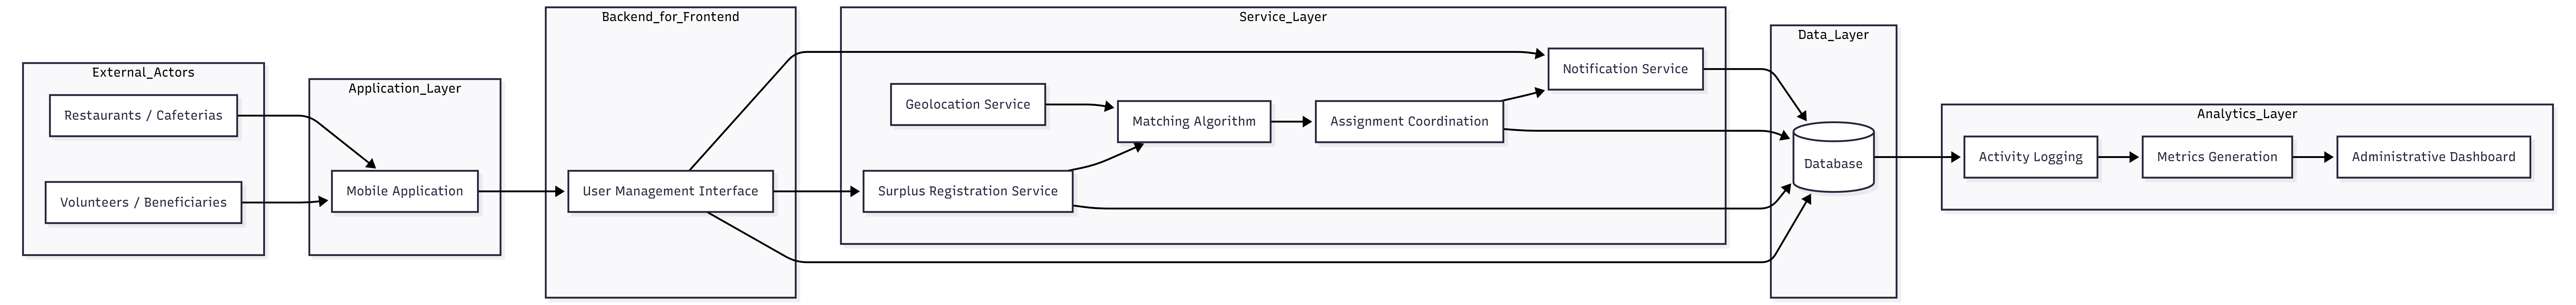
\includegraphics[width=\columnwidth]{System-Architecture-Change (1)}
  \caption{System architecture of the proposed food surplus redistribution platform.}
  \label{fig:architecture}
\end

The \textbf{External Actors} layer comprises two principal user groups: restaurants and cafeterias, which register surplus inventory as donors, and volunteers and beneficiaries, which include verified NGOs, student groups, and individual citizens who claim available donations.

The \textbf{Application Layer} hosts the Mobile Application and the User Management Interface, serving as the single point of interaction for all user types. It handles authentication, role assignment (donor, verified organization, or general beneficiary), and geographic eligibility verification.

The \textbf{Service Layer} is the core processing tier, composed of four components: the Surplus Registration Service validates and persists new food listings; the Geolocation Service enforces the 3\,km operational radius; the Matching Algorithm applies a priority queue favoring verified charitable organizations; and the Assignment Coordination module manages reservation states and expiry windows. A Notification Service dispatches tiered push alerts across all components.

The \textbf{Data Layer} consists of a centralized relational database that persists user profiles, food listings, geolocation records, assignment states, and transaction histories. The \textbf{Analytics Layer} extends from this database through an Activity Logging module, a Metrics Generation engine, and an Administrative Dashboard, enabling continuous impact reporting and system optimization.

\subsection{Matching and Priority Algorithm}

The core matching logic operates as a priority queue evaluated each time a new surplus listing is published. When a donor submits a listing, the algorithm: (1)~identifies all registered recipients within a 3\,km radius via the Geolocation Service; (2)~sorts them by a composite priority score that weights organizational verification status (verified NGO $>$ student group $>$ general user), historical pickup reliability, and geographic proximity; (3)~dispatches push notifications sequentially per tier with a 15-minute response window before cascading to the next level; and (4)~locks the listing upon pickup confirmation, removing it from the active pool.

\subsection{Operational Constraints}

The platform enforces strict boundaries to ensure food safety and logistical feasibility: (i)~listings must be published 2--4 hours before the donor's closing time; (ii)~pickups must be completed within 1--3 hours of publication; (iii)~listings expire automatically at midnight; and (iv)~the platform does not manage physical transport or quality certification, placing that responsibility on participating parties.

\subsection{Technology Stack}

The mobile application is developed using React Native for cross-platform support on Android and iOS, which is relevant given the Android-dominant market in Colombia. Backend services are implemented with Node.js exposing RESTful APIs. PostgreSQL with the PostGIS extension supports geospatial radius queries. Firebase Cloud Messaging (FCM) powers the real-time push notification pipeline. The stack is containerized with Docker and deployed on a cloud provider to ensure availability during peak usage windows.

\subsection{Evaluation Methodology}

System effectiveness will be assessed through an eight-week pilot deployment within the operational radius. Quantitative metrics include: total kilograms of food redistributed, number of successful donor--recipient matches per week, average time from listing publication to pickup confirmation, and notification response rates per priority tier. User experience will be measured via a post-pilot survey using a 5-point Likert scale covering usability, notification timeliness, and perceived social impact. Waste reduction estimates will be derived by multiplying successfully claimed listings by the average portion weight recorded at registration.

\subsection{System Architecture}

Figure~\ref{fig:architecture} presents the proposed system architecture.


\section{Results and Discussion}
\textbf{\textbf{The results presented in this section are based on a realistic projections constructed from the system parameters and boundaries defined in the Workshop 1 systems analysis. These represent the expected performance of the platform and will be validated through actual experiments, pilot deployment, and user testing in subsequent workshops (Workshop 3 and 4).}}

To evaluate the potential impact of the proposed platform, a simulated pilot scenario was constructed based on typical food surplus generation patterns observed in small urban restaurants and university cafeterias located near the Engineering Faculty of the Universidad Distrital Francisco José de Caldas. The evaluation considered three key performance indicators: surplus food recovery rate, number of successful redistributions, and estimated reduction in food waste.

\bibliographystyle{IEEEtran}
\bibliography{references} 


\section*{Acknowledgments}

\end{document}